\documentclass{standalone}
\usepackage[utf8]{inputenc}
\usepackage{tikz}

\usetikzlibrary{decorations, decorations.pathreplacing, decorations.pathmorphing}

\begin{document}

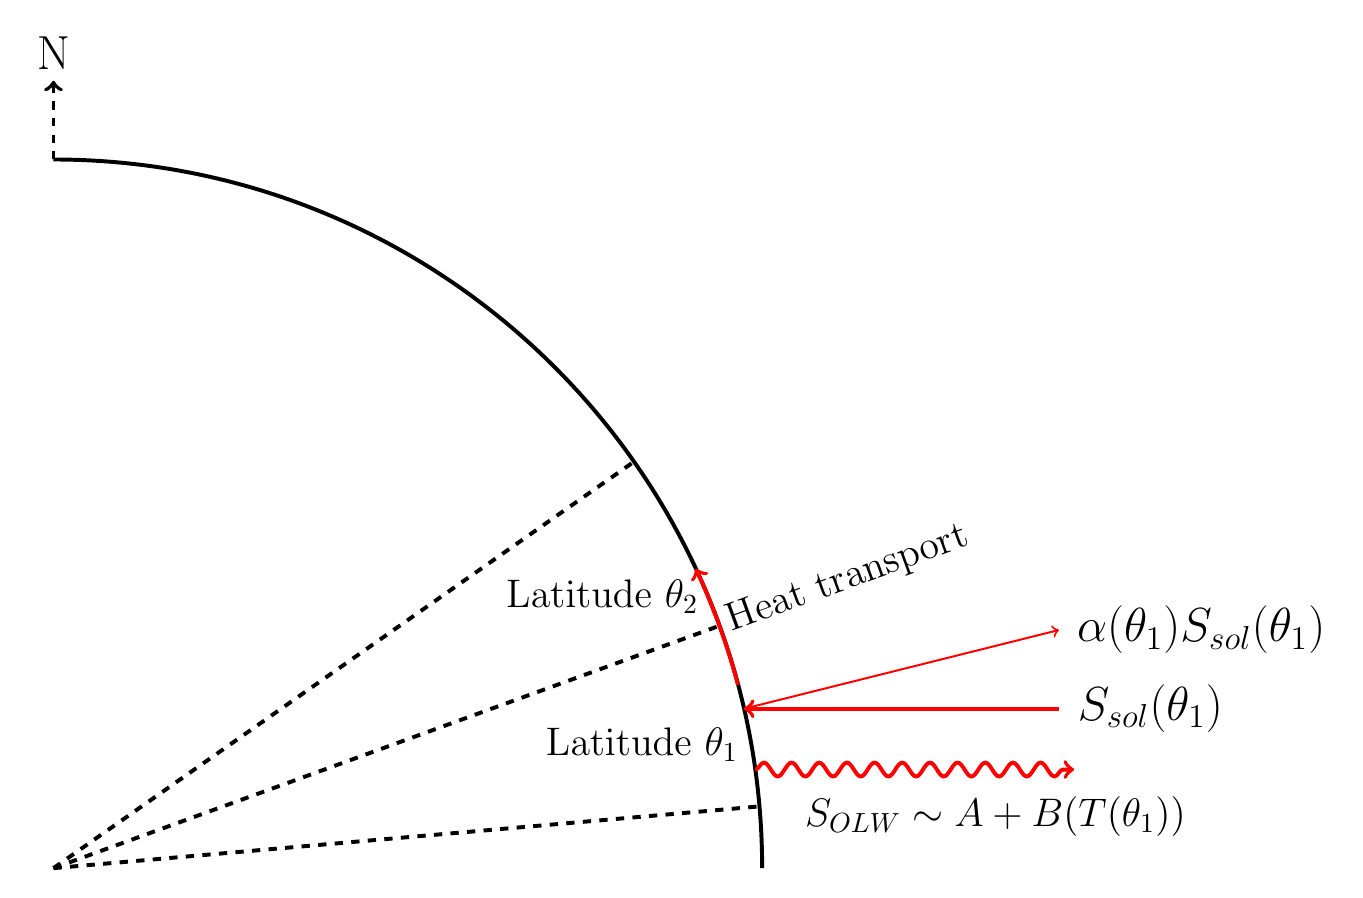
\begin{tikzpicture}
    \def\r{9}
    \def\t{20}
    \def\p{35}
    \def\w{0.5mm}
    \draw[line width = \w] (\r,0) arc[start angle = 0, end angle=90, radius = \r];

    \draw[->, dashed, line width = \w] (0,\r) -- (0,\r + 1) node[above]{\LARGE N};

    \draw[dashed, line width = \w] (0,0) -- ({\r * cos(5)},{\r * sin( 5 ) });
    \draw[dashed, line width = \w] (0,0) -- ({\r * cos(\t)},{\r * sin( \t ) });
    \draw[dashed, line width = \w] (0,0) -- ({\r * cos(\p)},{\r * sin( \p ) });

    %\draw[line width = 0.75*\w, ->] (2,0)  arc[start angle = 0, end angle = \t, radius = 2];
    %\draw[line width = 0.75*\w, ->] (3,0)   arc[start angle = 0, end angle = \p, radius = 3];

    %\draw ({1 * cos(\t/2)},{1* sin( \t/2 ) }) node[left]{\Large $\theta_1$};

    \draw[->, line width=\w, red ] ({\r * cos(\t /2 + 3) + 4},{\r * sin( \t /2 +3) }) node[right=1mm, black]{\LARGE $S_{sol}(\theta_1)$} -- ({\r * cos(\t /2 + 3) },{\r * sin( \t /2 +3 ) });
    \draw[->,line width=0.5*\w, red] ({\r * cos(\t /2 + 3) },{\r * sin( \t /2 + 3) }) -- ({\r * cos(\t /2+ 3) + 4},{\r * sin( \t /2 + 3) +1}) node[right=1mm, black] {\LARGE $\alpha(\theta_1)S_{sol}(\theta_1)$};

    \draw[->, decoration={snake}, decorate, red, line width=\w] ({\r * cos(\t /2 - 2) },{\r * sin( \t /2 - 2) }) -- ({\r * cos(\t /2 -2 ) + 4.05},{\r * sin( \t /2 -2)}) node[left=10mm, black, below=2mm] {\Large $S_{OLW}\sim A + B(T(\theta_1))$};

    \draw[red, ->, line width = \w] ({\r * cos(\t -5)},{\r * sin( \t -5 ) })  arc[start angle = \t-5, end angle=\t+5 , radius = \r];

    \draw ({\r * cos(\t)},{\r * sin( \t ) }) node[right,rotate= \t]{\Large Heat transport};

    %\draw ({\r * cos(\t/2-4)},{\r * sin( \t/2-4) }) node[left=25mm, above= -3mm, rotate=0]{\Large with $\alpha(\theta_1), \, T(\theta_1)$};

    \draw ({\r * cos(\t/2+1.5)},{\r * sin( \t/2) }) node[left, rotate=0]{\Large Latitude $\theta_1$};

    \draw ({\r * cos(\p/2+5)},{\r * sin( \p/2+5) }) node[left, rotate=0]{\Large Latitude $\theta_2$};
\end{tikzpicture}

\end{document}

